%!TEX TS-program = xelatex
%!TEX encoding = UTF-8 Unicode

\documentclass[12pt, a4paper]{scrartcl}

%% Page Layout
\usepackage[margin=1in]{geometry}

\usepackage{euler} % math font package needs to be loaded before others
\usepackage{xunicode,xltxtra, polyglossia}
\setdefaultlanguage[variant=american]{english}

%% fonts, symbols, text
	%%% fonts
	\usepackage{fontspec} %(include if mathspec is not loaded)
	\defaultfontfeatures{Mapping=tex-text, Ligatures=TeX}
	%%% text decoration
	\usepackage[normalem]{ulem} % sout
	%%% semantics symbols
	\usepackage{stmaryrd}
	\usepackage{amsmath,amssymb}
	\newcommand{\transl}{\rightsquigarrow \ensuremath}
	%%% other symbols
	\usepackage{pifont}% http://ctan.org/pkg/pifont
	\newcommand{\cmark}{\ding{51}}%
	\newcommand{\xmark}{\ding{55}}%

%% layout
%%% page layout
\usepackage{multicol}


%% bibliography
\usepackage[round]{natbib}
\newcommand{\posscite}[1]{\citeauthor{#1}'s (\citeyear{#1})}

%% figures, examples, diagrams
%%% examples
\usepackage{linguex}
\renewcommand{\firstrefdash}{}
%%% tables 
\usepackage{booktabs}
%%% figures
\usepackage{graphics}


%% decoration and features
%%% colors
\usepackage[dvipsnames]{xcolor}

%% bibliography
\renewcommand*{\refname}{\normalsize\textbf{References}\\ \vspace{-.5\baselineskip}}

%% fonts
\setmainfont[Scale=MatchLowercase,Mapping=tex-text, SmallCapsFeatures={Letters=SmallCaps}]{Times New Roman}
\setsansfont[Scale=MatchLowercase,Mapping=tex-text]{Times New Roman}

\usepackage{setspace}
\begin{document}

\bibliographystyle{plainnat}
% \enablehyphenation
% \vspace{-2em}
% \maketitle
\textcolor{white}{.} \vspace{-3.9\baselineskip} \\
\begin{center}
	\textbf{\large%\thetitle
		%A diverse family (of sentences)\\ 
		Projection differs across embedding operators---but not like you think}
\end{center}

\vspace*{-.4cm}

\noindent 
We present experimental evidence that i) the projection of the content of the clausal complement of attitude predicates varies across entailment-canceling operators (negation, question, modal, conditional) and ii) this by-operator variation differs across attitude predicates. Our results do not align with the long-standing distinction between factive and semi-factive predicates (see, e.g., \citealt{karttunen_observations_1971,djarv_cognitive_2018}). Instead, the observed by-operator variation groups predicates by lexical semantic/pragmatic properties that raise important questions for future research on projection.

\noindent
{\bf Projection across entailment-cancelling operators.} Interpreters may infer that a speaker who utters one of the attitude ascriptions in  \ref{ex:family} is committed to the truth of the content of the complement (CC), that Julian dances salsa, even though the complement occurs under an entailment-canceling operator, such as negation \ref{ex:neg}, a polar question \ref{ex:q}, a modal \ref{ex:mod}, or a conditional \ref{ex:cond}.

%	Certain attitude ascriptions come with an inference to the truth of their complement, even if embedded under entailment-cancelling operators (shown for \emph{discover} in \ref{ex:family}), in which case the inference is said to \emph{project} (e.g. \citealp{karttunen_observations_1971}).

	\vspace{-.3\baselineskip}
	\ex. \label{ex:family}
		\a. \label{ex:neg}
			Negation: \hfill
			\emph{\lq Cole didn't discover that Julian dances salsa.\rq}
		\b. \label{ex:q}
			Polar Question: \hfill
			\emph{\lq Did Cole discover that Julian dances salsa?\rq}
		\c. \label{ex:mod}
			Modal: \hfill
			\emph{\lq Perhaps Cole discovered that Julian dances salsa.\rq}
		\d. \label{ex:cond}
			Conditional: \hfill
			\emph{\lq If Cole discovered that Julian dances salsa, Logan will be joyful.\rq}
		\z.
	\z.

	\vspace{-.4\baselineskip}
	% Previous work on projection showed that it is not a categorial property of lexical triggers \citep{tonhauser_how_2018}, but a gradient one, affected by various contextual factors \citep{simons_what_2010,de_marneffe_did_2012,beaver_questions_2017,degen_prior_2021}. In light of this, we expect that the hetergeneous entailment-cancelling operators in \ref{ex:family} affect projection differentially.
	%
	\citealt{karttunen_observations_1971} suggested that the CC of factive predicates (e.g., \emph{regret, forget}) projects from under all four operators, whereas that of semi-factive predicates (e.g., \emph{discover, realize, see, notice}) always projects from under negation, but not always from under polar questions, modals, or conditionals. 
	
There has been, to date, one investigation of by-operator variation: \citealt{smith_relationship_2014}, who investigated by-operator variation (negation, conditional) for the projective content of six expressions (\emph{know, the, win}, epithets, clefs, non-restrictive relative clauses (NRRCs)), observed by-operator variation for some contents (e.g., that of \emph{know}, but not that of clefs) and that this by-operator variation differs across contents (e.g., the content of NRRCs was more projective under conditionals than negation, the opposite pattern was observed for \emph{win}). It is not clear, however, whether the response task used by \citealt{smith_relationship_2014} measured projection, as participants were asked to rate how surprised they would be to learn the content under investigation after observing the utterance.

There has not yet been an experimental investigation of by-operator variation between factive and semi-factive predicates. \citealt{djarv_cognitive_2018} and \citealt{tonhauser_how_2018} did, however, observe by-predicate projection variation under polar questions. \citealt{djarv_cognitive_2018} observed a difference between \emph{be happy} and \emph{appreciate} (which they assumed are factive predicates) and \emph{be aware} and \emph{realize} (which they assumed are semi-factive predicates). However, the response task (acceptability of an affirmation of the CC while the main clause content was denied) did not measure projection of the CC. \citealt{tonhauser_how_2018} measured projection of the CC of a broad range of attitude predicates from under polar questions: The by-predicate projection differences they observed did not align with what would be expected from Karttunen's classification (e.g., the CC of semi-factive \emph{realize} was as projective as that of factive \emph{be annoyed} and more projective than that of semi-factive \emph{discover}).

\noindent
{\bf Experiment.} We present the results of an experiment designed to investigate by-operator projection variation for the CCs of 20 attitude predicates, including purported factive and semi-factive predicates (e.g., \emph{be annoyed, discover}). Projection was measured for the same contents across all four operators in \ref{ex:family} using the `certain that' diagnostic for projection (see also, e.g., \citealt{tonhauser_how_2018, djaerv-bacovcin-salt27, mahler2020}). 


%In our work, we analyze measures from a task designed to measure speaker commitment more directly to address the questions: \textbf{(i)} Is projection affected by differences in entailment-canceling environments? \textbf{(ii)} Do these effects vary for different triggers (and in what way)? We used a response task to elicit judgments about how strongly a speaker would be committed towards the embedded clause \citep[from][]{tonhauser_prosodic_2016}. We presented sentences like in \ref{ex:family} as asserted by a named speaker (e.g. “\textbf{Daniel:} \emph{\lq Did Cole\dots?\rq}”). Participants then provided a certainty-rating in response to a prompt like: \emph{“Is Daniel certain that Julian dances salsa?”}, by moving a slider on a scale from \lq no\rq\ (coded as \texttt{0}), to \lq yes\rq\ (coded as \texttt{1}). 

% paragraph experiment (end)
\noindent
{\bf Methods and expectations.} Projection of the CC of the 20 attitude predicate was measured in four sets of experiments: The attitude predicates were embedded under polar questions in Exps.~1, under negation in Exps.~2, under {\em perhaps} in Exps.~3, and in the antecedent of a conditional in Exps.~4. (Each set of experiments consisted of three experiments that differed in the at-issueness measure used in a separate block. We focus on the projection ratings here.) In each experiment, participants were asked to read utterances like those in \ref{ex:family} and judge whether the speaker (who was named) was certain of the CC (e.g.: Is [the speaker] certain that Julian dances salsa?). Participants gave their response on a slider marked `no' (coded as 0) at one and and `yes' (coded as 1) on the other end. Each participant rated the projection of the CC of all 20 attitude predicates (each paired with a unique content from a set of 20 contents) under one operator. We analyze the data from 2,682 self-reported native speakers of American English recruited on Prolific or Amazon's MT platform. We expect the CC of factive predicates to consistently receive relatively high projection ratings under all four operators, and the CC of semi-factive predicates to exhibit high projection ratings under negation and possibly lower ratings under the other operators.

%We compared certainty-ratings for the four entailment-canceling operators in \ref{ex:family}, and 20 clause-embedding predicates (\texttt{verb}: {\em be annoyed, discover, know, reveal, see, acknowledge, admit, announce, confess, confirm, establish, hear, inform, prove, pretend, suggest, say, think, be right, demonstrate}).
%	Based on the Karttunen-Djärv generalization about emotive factives vs. cognitive semi-factives, we would expect emotive factives (\emph{be annoyed}), and verbs normally taken to be factive (\emph{know}), to be highly projective in a way that is indifferent to the embedding context, and cognitive semi-factives (\emph{discover, see}) to show higher projectivity ratings under negation compared to questions and conditionals.

%The study, originally designed to address a different research question, consisted of 12 experiments, all of which manipulated the factor \texttt{verb} for 20 items corresponding to to the content of the complement clause. Experiments 1--3 used polar question embedding, exps. 4--6 used negation, 7--9 modals, and 10--12 conditionals, making the \texttt{operator} manipulation a between-subjects factor. 

%We analyzed data from 2682 self-identified native English speakers participated online across the 12 experiments (recruited via Prolific and Amazon MTurk). Participants saw items Latin-squared and randomized with six control stimuli.

% paragraph method (end)

\noindent
{\bf Results.} Fig.~\ref{fig:figure1} plots the mean projection ratings for the 20 attitude predicates by embedding operator; the predicates are ordered by their mean projection across all operators (\emph{be annoyed} has the highest overall projection mean). We observe by-operator variation in projection means as well as differences across the predicates in by-operator variation: For instance, whereas the CC of \emph{be annoyed} projects more from under questions and negation than from under conditionals and modals, the CC of \emph{know} projects more from under questions than from under conditionals and negation, and the CC of \emph{discover} projects more from under questions and conditionals than from under negation and modals. These results are not aligned with the distinction between factive and semi-factive predicates proposed in \citealt{karttunen_observations_1971} or assumed in \citealt{djarv_cognitive_2018}: Contrary to assumption, the CC of the purportedly factive predicate \emph{be annoyed} does not project invariably from all four operators, and the CC of the purportedly semi-factive predicate \emph{discover} does not project more from under negation than the other three operators. For {\em know}, we observe a third pattern -- one that is not aligned with a classification as a factive nor as a semi-factive predicate. 

==== THIS IS AS FAR AS I've COME ====

	% \vspace{-.3\baselineskip}
	% \textbf{version w baseline know/m}
	% \noindent The data was analyzed using a mixed effects linear regression (using \texttt{lme4, lmertest} in \texttt{R}; \citealp{bates_fitting_2015,kuznetsova_lmertest_2016,r_core_team_r_2014}), with \texttt{know} and \texttt{modal} as reference levels, and random intercepts for participants and items. We found highly significant main effects of \texttt{operator} (\texttt{conditional}: $+0.142$, \texttt{negation}: $+0.143$, ; \texttt{question}: $+0.225$, where $p < 2e^{-16}$ in all three cases), as well as many interactions of \texttt{operator} and  \texttt{verb} across the board (where $p < 0.001$ in $38$ cases, $p < 0.01$ in one, and $p < 0.05$ in three out of $57$ possible interactions).\\

	\noindent The data was analyzed using a mixed effects linear regression (using \texttt{lme4, lmertest} in \texttt{R}; \citealp{bates_fitting_2015,kuznetsova_lmertest_2016,r_core_team_r_2014}), with \texttt{be\_annoyed} and \texttt{negation} as reference levels, and random intercepts for participants and items.
	% The mean for this baseline (intercept) is $0.867$.
	We found highly significant main effects of \texttt{operator}: For our baseline \texttt{be\_annoyed}, both \texttt{conditional} and \texttt{modal} are clearly less projective than negation, thereby supporting the claim that the embedding context does matter. We also found many interactions of \texttt{operator} and \texttt{verb} across the board, suggesting that the effect of embedding context diffes by verb. Notably, \emph{\lq discover\rq} is more projective in polar questions and conditional antecedents than under negation, patterning opposite to Karttunen's claims about semi-factives. For the emotive predicate \emph{\lq be annoyed\rq} no significant effect is found for \texttt{question} (vs \texttt{negation}), as would be expected based on Karttunen, but we do find unexpected differences between \texttt{negation} $>$ \texttt{conditional, modal}. \emph{know} shows effects that would be incompatible with a characterization as either factive or semi-factive: $\texttt{question} > \texttt{conditional, negation} > \texttt{modal}$. If \emph{\lq know\rq} is a factive predicate, no difference would be expected. If it is semi-factive, we would, again, expect higher projectivity under negation than in questions and conditionals.
	


	% for \texttt{conditional} ($-0.116$, $p < 1.6e^{-13}$) and \texttt{modal} ($-0.156$, $p < 2e^{-16}$), while the effect of \texttt{question} was only marginally significant ($+0.025$, $p < 0.1$). We also found many interactions of \texttt{operator} and \texttt{verb} across the board (where $p < 0.001$ in $43$ cases, $p < 0.01$ in three, and $p < 0.05$ in one out of $57$ possible interactions).\\
	
% paragraph results (end)

\noindent
{\bf Discussion.} 

We observe that projection varies by predicate (e.g., the CC of \emph{be annoyed} is more projective than that of \emph{discover}; replicating the results of  \citealt{degen-tonhauser-language}). 

No categorical distinction between factive and non-factive predicates either


add discussion about verb classes here


\newpage

\begin{figure}[t]
		\vspace{-.8\baselineskip}
		\centering
		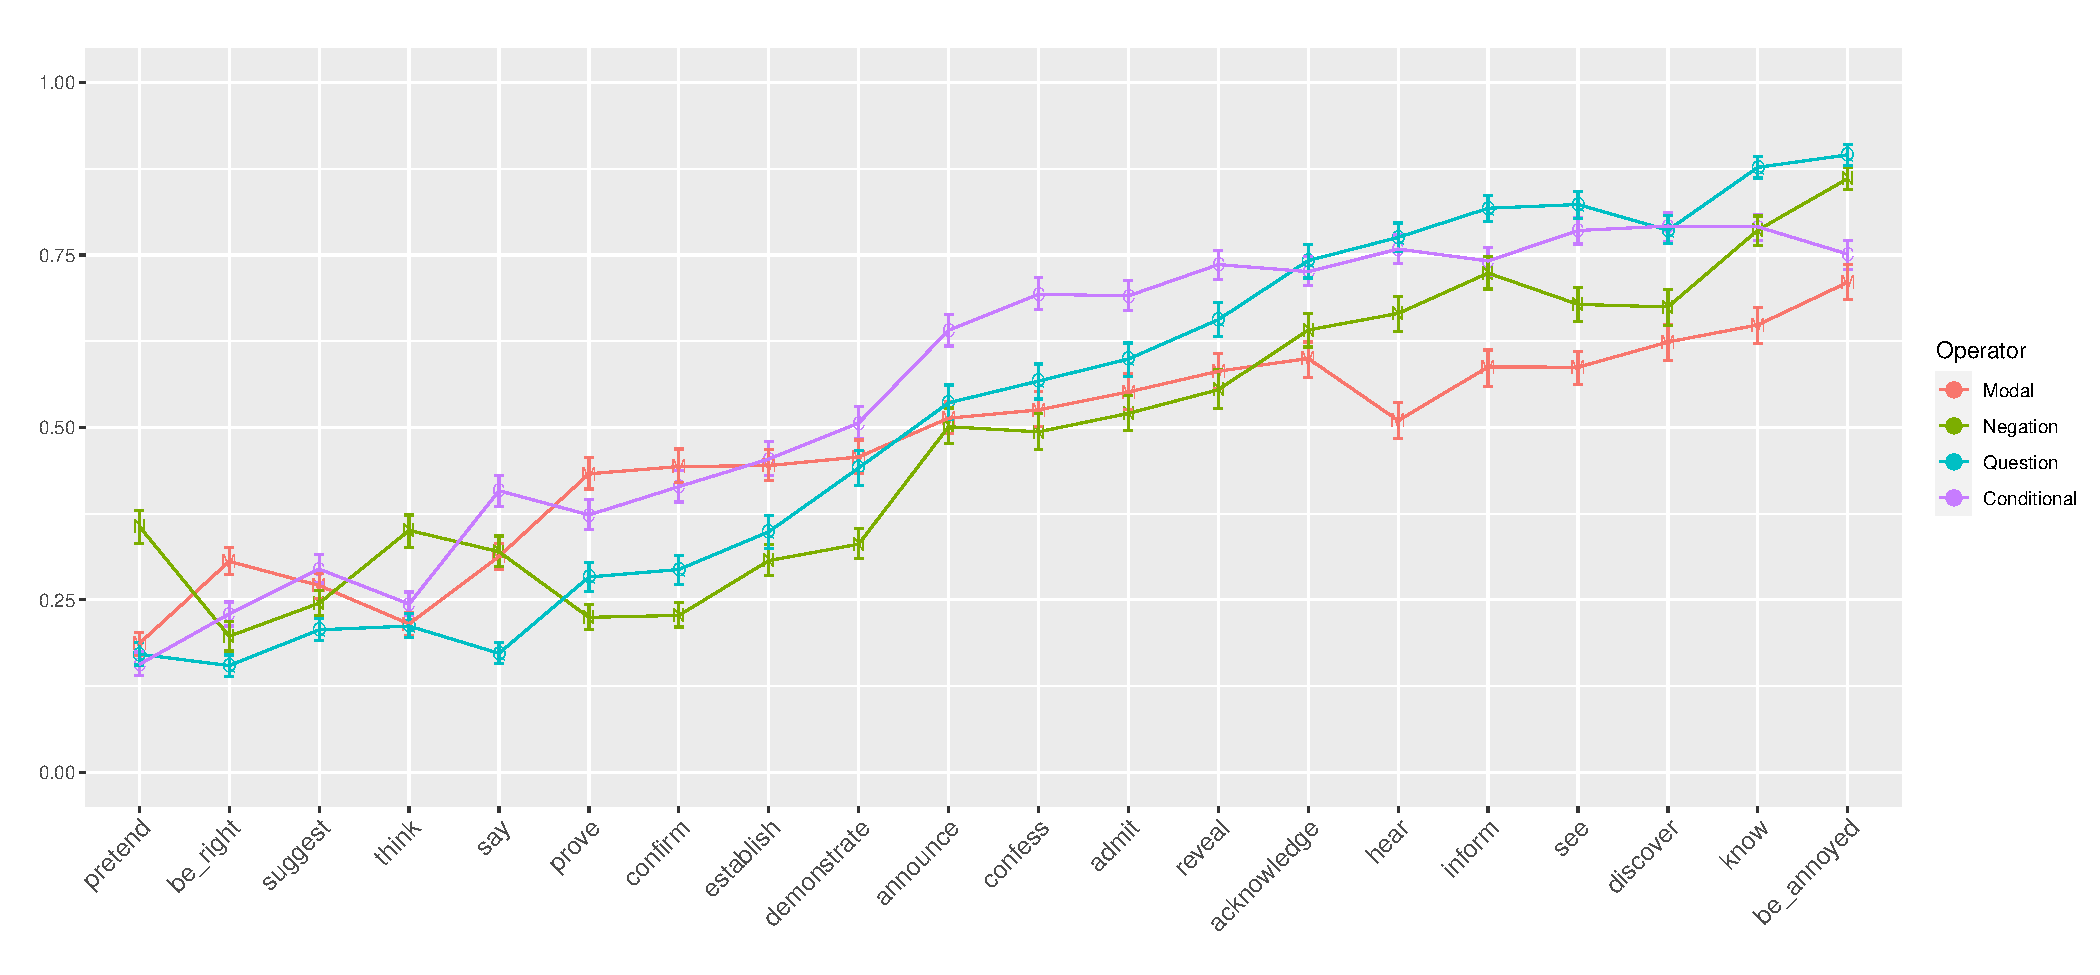
\includegraphics[width=\textwidth]{graphs/proj-by-both.pdf}\vspace{-1.2\baselineskip}
		\caption{\small Mean certainty ratings by predicate and operator with 95\% bootstrapped confidence intervals. Embedding operator coded by letter and color:  \texttt{N} (blue): negation, \texttt{M} (green): modals, \texttt{C} (red): conditional antecedents, \texttt{Q} (purple): polar questions.}
		\label{fig:figure1}
	\end{figure}

\newpage

\bibliography{projective-content.bib}

\end{document}